% !TEX root = calculus.tex
\chapter{INFINITE NUMERICAL SEQUENCE}
\label{infinite-seq}
{\parindent=0pt
\athr Let us start our discussions of calculus by considering the definition of an \emph{infinite numerical sequence} or simply a \emph{sequence}.

We shall consider the following examples of sequences:
\begin{align}%
 1, \, 2, \, 4, \, 8, \, 16, \, 32, \, 64, \, 128, \, \ldots \label{series-01}\\
 5, \, 7, \, 9, \, 11, \, 13, \, 15, \, 17, \, 19, \, \ldots \label{series-02}\\
1, \, 4, \, 9, \, 16, \, 25, \, 36, \, 49, \, 64, \, \ldots \label{series-03}\\
1,\, \sqrt{2}, \, \sqrt{3}, \, 2, \, \sqrt{5}, \, \sqrt{6}, \, \sqrt{7}, \, 2 \sqrt{2}, \, \ldots \label{series-04}\\
\frac{1}{2}, \,\frac{2}{3}, \,\frac{3}{4}, \,\frac{4}{5}, \,\frac{5}{6}, \,\frac{6}{7}, \,\frac{7}{8}, \,\frac{8}{9}, \, \ldots \label{series-05}\\
2, \, 0, \, - 2, \, - 4, \, - 6, \, - 8, \, - 10, \, - 12, \, \ldots \label{series-06}\\
1, \frac{1}{2}, \,\frac{1}{3}, \,\frac{1}{4}, \,\frac{1}{5}, \,\frac{1}{6}, \,\frac{1}{7}, \,\frac{1}{8}, \, \ldots \label{series-07}\\
1, \frac{1}{2}, \, 3, \, \frac{1}{4}, \, 5, \,\frac{1}{6}, \, 7, \,\frac{1}{8}, \, \ldots \label{series-08}\\
1, \, -1, \, \frac{1}{3}, \, -\frac{1}{3}, \, \frac{1}{5}, \, -\frac{1}{5}, \, \frac{1}{7}, \, -\frac{1}{7}, \, \ldots \label{series-09}\\
1, \frac{2}{3}, \,\frac{1}{3}, \,\frac{1}{4}, \,\frac{1}{5}, \,\frac{6}{7}, \,\frac{1}{7}, \,\frac{8}{9}, \, \ldots \label{series-10}
\end{align}
Have a closer look at these examples. What do they have in common?

\rdr It is assumed that in each example there must be an infinite number of terms in a sequence. But in general, they are all different.

\athr In each example we have eight terms of a sequence. Could you write, say, the ninth term?

\rdr Sure, in the first example the ninth term must be 256, while in the second example it must be 21.

\athr Correct. It means that in all the examples there is a \emph{certain law}, which makes it possible to write down the ninth, tenth, and other terms of the sequences. Note, though, that if there is a \emph{finite number} of terms in a sequence, one may fail to discover the law which governs the infinite sequence.

\rdr Yes, but in our case these laws are easily recognizable. In example \eqref{series-01} we have the terms of an infinite geometric progression with common ratio 2. In example \eqref{series-02} we notice a sequence of odd numbers starting from 5. In example \eqref{series-03} we recognize a sequence of squares of natural numbers.

\athr Now let us look at the situation more rigorously. Let us enumerate all the terms of the sequence in sequential order, i.e. $1, \, 2, \, 3, \ldots, \,n, \ldots$  There is a certain law (a rule) by which each of these natural numbers is \emph{assigned} to a certain number (the corresponding term of the sequence). In example \eqref{series-01} this arrangement is as follows:
{\smaller \begin{center}
\begin{tabular}{cccccccccl}
\noalign{\global\arrayrulewidth=.5mm}
  \arrayrulecolor{DodgerBlue}
\hline
1 & 2 & 4 & 8 & 16 & 32 & \ldots & $2^{n-1}$ & \ldots & (terms of the sequence) \\
$\uparrow$ & $\uparrow$ & $\uparrow$ & $\uparrow$ & $\uparrow$ & $\uparrow$ &  & $\uparrow$ &  &   \\
1 & 2 & 3 & 4 & 5 & 6 & \ldots & $n$ & \ldots & (position numbers of the terms)\\
\hline
\end{tabular}
\end{center}}
In order to describe a sequence it is sufficient to indicate the term of the sequence corresponding to the number $n$, i.e. to write down the term of the sequence occupying the nth position. Thus, we can formulate the following definition of a sequence. 
\begin{mytheo}{Definition}
We say that there is an infinite numerical sequence if every
natural number (position numbers is unambiguously placed in correspondence with a definite number (term of the sequence) by a specific rule.
\end{mytheo}
This relationship may be presented in the following general form:
{\smaller \begin{center}
\begin{tabular}{cccccccc}
\noalign{\global\arrayrulewidth=.5mm}
  \arrayrulecolor{DodgerBlue}
\hline
$y_{1}$ & $y_{2}$ & $y_{3}$ & $y_{4}$ & $y_{5}$ & \ldots & $y_{n}$ & \ldots \\
$\uparrow$ & $\uparrow$ & $\uparrow$ & $\uparrow$ & $\uparrow$ &    & $\uparrow$  &   \\
1 & 2 & 3 & 4 & 5 & \ldots & $n$ & \ldots  \\ 
 \hline
\end{tabular}
\end{center}}
'The number $y_{n}$  is the $n$th term of the sequence, and the whole sequence is sometimes denoted by a symbol ($y_{n}$).

\rdr We have been given a somewhat different definition of a sequence: a sequence is a function defined on a set of natural numbers (integers).

\athr Well, actually the two definitions are equivalent. However, I am not inclined to use the term ``function'' too early. First, because the discussion of a function will come later. Second, you will normally deal with somewhat
different functions, namely those defined not on a set of integers but on the real line or within its segment. Anyway, the above definition of a sequence is quite correct.

Getting back to our examples of sequences, let us look in each case for an \emph{analytical expression (formula)} for the $n$th term. Go ahead.

\rdr Oh, this is not difficult. In example \eqref{series-01} it is $y_{n}=2^{n}$. In \eqref{series-02} it is  $y_{n}=2n+3$. In \eqref{series-03} it is  $y_{n}= n^{2}$. In \eqref{series-04} it is  $y_{n}= \sqrt{n}$. In \eqref{series-05} it is  $y_{n}=1 - \dfrac{1}{n+1}= \dfrac{n}{n+1}$. In \eqref{series-06} it is  $y_{n}=4- 2n$. In \eqref{series-07} it is  $y_{n}= \dfrac{1}{n}$.

In the remaining three examples I just do not know. 

\athr Let us look at example \eqref{series-08}. One can easily see that if $n$ is an even integer, then $y_{n}=\dfrac{1}{n}$, but if $n$ is odd, then $y_{n} = n$, It means that 
\begin{equation*}%
y_{n}= 
\begin{cases}
\dfrac{1}{n} \,\, \text{if} \,\, n=2k \\
n  \,\, \text{if} \,\, n= 2k-1
\end{cases}
\end{equation*}
\rdr Can I, in this particular case, find a single analytical expression for $y_{n}$?

\athr Yes, you can. Though I think you needn't. Let us present $y_{n}$ in a different form:
\begin{equation*}%
y_{n} = a_{n} n + b_{n} \frac{1}{n}
\end{equation*}
and demand that the coefficient $a_{n}$ be equal to unity if $n$ is odd, and to zero if $n$ is even; the coefficient $b_{n}$ should behave in quite an opposite manner. In this particular case these coefficients can be determined as follows:
\begin{equation*}%
%\begin{split}
a_{n}  = \frac{1}{2} \left[1 - (-1)^{n} \right], \quad b_{n}  =  \frac{1}{2} \left[1 + (-1)^{n} \right] 
%\end{split}
\end{equation*}
Consequently 
\begin{equation*}%
y_{n}  = \frac{n}{2} \left[1 - (-1)^{n} \right]+  \frac{1}{2n} \left[1 + (-1)^{n} \right] 
\end{equation*}
Do in the same manner in the other two examples. 

\rdr For sequence  \eqref{series-09} I can write
\begin{equation*}%
y_{n}  = \frac{1}{2n} \left[1 - (-1)^{n} \right]+  \frac{1}{2(n-1)} \left[1 + (-1)^{n} \right] 
\end{equation*}
and for sequence \eqref{series-10}
\begin{equation*}%
y_{n}  = \frac{1}{2n} \left[1 - (-1)^{n} \right]+  \frac{n}{2(n+1)} \left[1 + (-1)^{n} \right] 
\end{equation*}

\athr It is important to note that an analytical expression for the nth term of a given sequence is not necessarily a unique method of defining a sequence. A sequence can be defined, for example, by \emph{recursion} (or the \emph{recurrence method}) (Latin word \emph{recurrere} means to run back). In this case, in order to define a sequence one should describe the first term (or the first several terms) of the sequence and a recurrence (or a recursion) relation, which is an expression for the $n$th term of the sequence via the preceding one (or several preceding terms).

Using the recurrence method, let us present sequence \eqref{series-01}, as follows
\begin{equation*}%
y_{1	} = 1, \quad y_{n}  = 2  y_{n - 1}  
\end{equation*}

\rdr It's clear. Sequence \eqref{series-02} can be apparently represented by formulas 
\begin{equation*}%
y_{1	} = 5, \quad y_{n}  = y_{n - 1}  + 2
\end{equation*}

\athr That's right. Using recursion, let us try to determine one interesting sequence
\begin{equation*}%
y_{1	} = 1, \quad y_{2} = 1, \quad y_{n}  =   y_{n - 2} +   y_{n - 1}  
\end{equation*}
\begin{equation}%
1, \, 1, \, 2, \, 3, \, 5, \, 8, \, 13, \, 21, \ldots
\label{fibonacci}
%eq-11
\end{equation}
This sequence is known as the \emph{Fibonacci sequence} (or \emph{numbers}).

\rdr I understand, I have heard something about. the problem of Fibonacci rabbits.

\athr Yes, it was this problem, formulated by Fibonacci, the 13th century Italian mathematician, that gave the name to this sequence \eqref{fibonacci}. The problem reads as follows. A man places a pair of newly born rabbits into a warren and wants to know how many rabbits he would have over a certain period of time. A pair of rabbits will start producing offspring two months after they were born and every following month one new pair of rabbits will appear. At the beginning (during the first month) the man will have in his warren only one pair of rabbits ($y_{1} = 1$); during the second month he will have the same pair of rabbits ($y_{2} = 1$); during the third month the offspring will appear, and therefore the number of the pairs of rabbits in the warren will grow to two ($y_{3} = 3$); during the fourth month there will be one more reproduction of the first pair ($y_{4} = 3$); during the fifth month there will be offspring both from the first and second couples of rabbits ($y_{5} = 5$), etc. An increase of the number of pairs in the warren from month to month is plotted in \fig{fig-01}. One can see that the numbers of pairs of rabbits counted at the end of each month form sequence \eqref{fibonacci}, i.e. the Fibonacci, sequence.

\begin{figure}[!h]
\centering
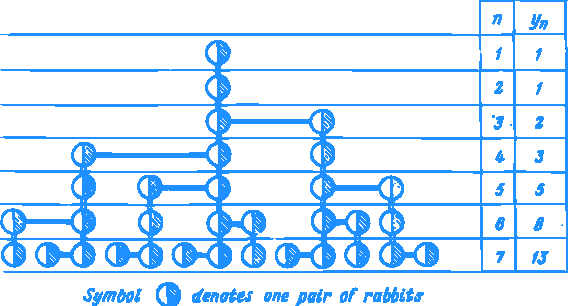
\includegraphics[width=0.9\textwidth]{figures/fig-01.pdf}
\caption{Visualising Fibonacci rabbits.}
\label{fig-01}
\end{figure}

\rdr But in reality the rabbits do not multiply in accordance with such an idealized pattern. Furthermore, as time goes on, the first pairs of rabbits should obviously stop proliferating.

\athr The Fibonacci sequence is interesting not because it describes a simplified growth pattern of rabbits' population. It so happens that this sequence appears, as if by magic, in quite unexpected situations. For example, the Fibonacci numbers are used to process information by computers and to optimize programming for computers. However, this is a digression from our main topic.

Getting back to the ways of describing sequences, I would like to point out that the \emph{very method chosen to describe a sequence is not of principal importance}. One sequence may be described, for the sake of convenience, by a formula for the $n$th term, and another (as, for example, the Fibonacci sequence), by the recurrence method. What is important, however, is the method used to describe the \emph{law of correspondence}, i.e. the law by which any natural number is placed in correspondence with a certain term of the sequence. In a number of cases such a law can be formulated only by words. The examples of such cases are shown below:
\begin{align}%
2, \, 3, \, 5, \, 7, \, 11, \, 13, \, 17, \, 19, \, 23, \ldots \label{series-12}\\
3,  \, 3.1, \,  3.14, \,  3.141, \,  3.1415, \,  3.14159, \ldots \label{series-13}
\end{align}

In both cases we cannot indicate either the formula for the- nth term or the recurrence relation. Nevertheless, you can without great difficulties identify specific laws of correspondence and put them in words.

\rdr Wait a minute. Sequence \eqref{series-12} is a sequence of \emph{prime numbers} arranged in an increasing order, while \eqref{series-13} is, apparently, a sequence composed of decimal approximations, with deficit, for $\pi$.

\athr You are absolutely right.

\rdr It may seem that a numerical sequence differs from a random set of numbers by a presence of an intrinsic \emph{degree of order} that is reflected either by the formula for tho $n$th term or by the recurrence relation. However, the last two examples show that such a degree of order needn't. be present.
%\begin{figure}[!h]
%\centering
%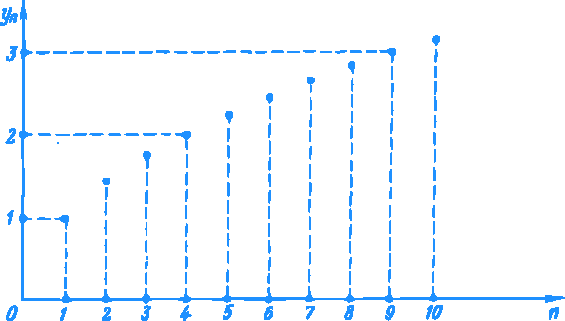
\includegraphics[width=0.9\textwidth]{figures/fig-02.pdf}
%\caption{Graph of the series \eqref{series-04}.}
%\label{fig-02}
%\end{figure}

\begin{figure}[!h]
\centering
\begin{tikzpicture}[line cap=round,line join=round,>=triangle 45,x=1.0cm,y=1.0cm]
%\filldraw[->,color=black] (-0.8900469095523698,0.) -- (11.877941351923667,0.);
\foreach \x in {,1,2,3,4,5,6,7,8,9,10}
\filldraw[shift={(\x,0)},color=black] (0pt,2pt) -- (0pt,-2pt) node[below] {\footnotesize $\x$};
%\filldraw[->,color=black] (0.,-0.9081072000876554) -- (0.,6.37592544744293);
\foreach \y in {0,1,2,3}
\filldraw[shift={(0,\y)},color=black] (2pt,0pt) -- (-2pt,0pt) node[left] {\footnotesize $\y$};
%\filldraw[color=black] (0pt,-10pt) node[below] {\footnotesize $0$};
\clip(-0.8900469095523698,-0.9081072000876554) rectangle (11.5,4);
\draw[color=black] (0,3.5) node[left] { $y_{n}$};
\draw[color=black] (11,0) node[below] { $n$};
\filldraw [line width=0.5pt,dash pattern=on 3pt off 3pt,color=DarkGray] (1.,1.)-- (1.,0.);
\filldraw [line width=0.5pt,dash pattern=on 3pt off 3pt,color=DarkGray] (2.,1.4142135623730951)-- (2.,0.);
\filldraw [line width=0.5pt,dash pattern=on 3pt off 3pt,color=DarkGray] (3.,1.7320508075688772)-- (3.,0.);
\filldraw [line width=0.5pt,dash pattern=on 3pt off 3pt,color=DarkGray] (4.,2.)-- (4.,0.);
\filldraw [line width=0.5pt,dash pattern=on 3pt off 3pt,color=DarkGray] (5.,2.23606797749979)-- (5.,0.);
\filldraw [line width=0.5pt,dash pattern=on 3pt off 3pt,color=DarkGray] (6.,2.449489742783178)-- (6.,0.);
\filldraw [line width=0.5pt,dash pattern=on 3pt off 3pt,color=DarkGray] (7.,2.6457513110645907)-- (7.,0.);
\filldraw [line width=0.5pt,dash pattern=on 3pt off 3pt,color=DarkGray] (8.,2.8284271247461903)-- (8.,0.);
\filldraw [line width=0.5pt,dash pattern=on 3pt off 3pt,color=DarkGray] (1.,1.)-- (0.,1.);
\filldraw [line width=0.5pt,dash pattern=on 3pt off 3pt,color=DarkGray] (4.,2.)-- (0.,2.);
\filldraw [line width=0.5pt,dash pattern=on 3pt off 3pt,color=DarkGray] (9.,3.)-- (9.,0.);
\filldraw [line width=0.5pt,dash pattern=on 3pt off 3pt,color=DarkGray] (9.,3.)-- (0.,3.);
\filldraw [line width=0.5pt,dash pattern=on 3pt off 3pt,color=DarkGray] (10.,3.1622776601683795)-- (10.,0.);
\filldraw [->,line width=1.2pt,color=DarkGray] (0.,0.) -- (0.,3.75);
\filldraw [->,line width=1.2pt,color=DarkGray] (0.,0.) -- (11,0);
\begin{scriptsize}
\filldraw [IndianRed] (1.,1.) circle (2.5pt);
\filldraw [IndianRed] (2.,1.4142135623730951) circle (2.5pt);
\filldraw [IndianRed] (3.,1.7320508075688772) circle (2.5pt);
\filldraw [IndianRed] (4.,2.) circle (2.5pt);
\filldraw [IndianRed] (5.,2.23606797749979) circle (2.5pt);
\filldraw [IndianRed] (6.,2.449489742783178) circle (2.5pt);
\filldraw [IndianRed] (7.,2.6457513110645907) circle (2.5pt);
\filldraw [IndianRed] (8.,2.8284271247461903) circle (2.5pt);
\filldraw [DodgerBlue] (1.,0.) circle (2.5pt);
\filldraw [DodgerBlue] (2.,0.) circle (2.5pt);
\filldraw [DodgerBlue] (3.,0.) circle (2.5pt);
\filldraw [DodgerBlue] (4.,0.) circle (2.5pt);
\filldraw [DodgerBlue] (5.,0.) circle (2.5pt);
\filldraw [DodgerBlue] (6.,0.) circle (2.5pt);
\filldraw [DodgerBlue] (7.,0.) circle (2.5pt);
\filldraw [DodgerBlue] (8.,0.) circle (2.5pt);
\filldraw [DodgerBlue] (0.,1.) circle (2.5pt);
\filldraw [DodgerBlue] (0.,2.) circle (2.5pt);
\filldraw [IndianRed] (9.,3.) circle (2.5pt);
\filldraw [IndianRed] (10.,3.1622776601683795) circle (2.5pt);
\filldraw [DodgerBlue] (9.,0.) circle (2.5pt);
\filldraw [DodgerBlue] (0.,3.) circle (2.5pt);
\filldraw [DodgerBlue] (10.,0.) circle (2.5pt);
\end{scriptsize}
\end{tikzpicture}
%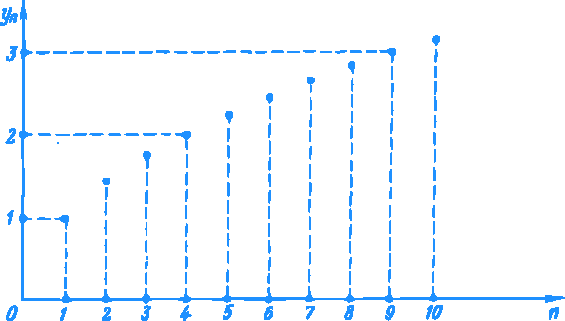
\includegraphics[width=0.9\textwidth]{figures/fig-02.pdf}
\caption{Graph of the series \eqref{series-04}.}
\label{fig-02}
\end{figure}

\athr Actually, a degree of order determined by a formula (an analytical expression) is not mandatory. It is important, however, to have a law (a rule, a characteristic) of correspondence, which enables one to relate any natural number to a certain term of a sequence. In examples \eqref{series-12} and \eqref{series-13} such laws of correspondence are obvious. Therefore,
\eqref{series-12} and \eqref{series-13} are not inferior (and not superior) to sequences \eqref{series-01}-\eqref{fibonacci} which permit an analytical description.
 \begin{figure}[!h]
\centering
\begin{tikzpicture}[line cap=round,line join=round,>=triangle 45,x=1.0cm,y=3.5cm]
\foreach \x in {,1,2,3,4,5,6,7,8,9,10}
\draw[shift={(\x,0)},color=black] (0pt,2pt) -- (0pt,-2pt) node[below] {\footnotesize $\x$};
\foreach \y in {,0,1}
\draw[shift={(0,\y)},color=black] (2pt,0pt) -- (-2pt,0pt) node[left] {\footnotesize $\y$};
%\draw[color=black] (0pt,-10pt) node[right] {\footnotesize $0$};
\draw[color=black] (0,1.2) node[left] { $y_{n}$};
\draw[color=black] (11,0) node[below] { $n$};
\clip(-0.7,-0.10) rectangle (11.5,1.3);
\draw [line width=1pt,color=IndianRed,dash pattern=on 3pt off 3pt,domain=0:11.5] plot(\x,{(--1.-0.*\x)/1.});
\draw [->,line width=1.2pt,color=DarkGray] (0.,0.) -- (0.,1.3);
\draw [->,line width=1.2pt,color=DarkGray] (0.,0.) -- (11.,0.);
\draw [line width=.75pt,dash pattern=on 3pt off 3pt,color=DarkGray] (1.,0.5)-- (1.,0.);
\draw [line width=.75pt,dash pattern=on 3pt off 3pt,color=DarkGray] (2.,0.6666666666666666)-- (2.,0.);
\draw [line width=.75pt,dash pattern=on 3pt off 3pt,color=DarkGray] (3.,0.75)-- (3.,0.);
\draw [line width=.75pt,dash pattern=on 3pt off 3pt,color=DarkGray] (4.,0.8)-- (4.,0.);
\draw [line width=.75pt,dash pattern=on 3pt off 3pt,color=DarkGray] (5.,0.8333333333333334)-- (5.,0.);
\draw [line width=.75pt,dash pattern=on 3pt off 3pt,color=DarkGray] (6.,0.8571428571428571)-- (6.,0.);
\draw [line width=.75pt,dash pattern=on 3pt off 3pt,color=DarkGray] (7.,0.875)-- (7.,0.);
\draw [line width=.75pt,dash pattern=on 3pt off 3pt,color=DarkGray] (8.,0.8888888888888888)-- (8.,0.);
\draw [line width=.75pt,dash pattern=on 3pt off 3pt,color=DarkGray] (9.,0.9)-- (9.,0.);
\draw [line width=.75pt,dash pattern=on 3pt off 3pt,color=DarkGray] (10.,0.9090909090909091)-- (10.,0.);
\begin{scriptsize}
\filldraw [DodgerBlue] (1.,0.) circle (2.5pt);
\filldraw [DodgerBlue] (2.,0.) circle (2.5pt);
\filldraw [DodgerBlue] (3.,0.) circle (2.5pt);
\filldraw [DodgerBlue] (4.,0.) circle (2.5pt);
\filldraw [DodgerBlue] (5.,0.) circle (2.5pt);
\filldraw [DodgerBlue] (6.,0.) circle (2.5pt);
\filldraw [DodgerBlue] (7.,0.) circle (2.5pt);
\filldraw [DodgerBlue] (8.,0.) circle (2.5pt);
\filldraw [DodgerBlue] (0.,1.) circle (2.5pt);
\filldraw [DodgerBlue] (9.,0.) circle (2.5pt);
\filldraw [DodgerBlue] (0.,3.) circle (2.5pt);
\filldraw [DodgerBlue] (10.,0.) circle (2.5pt);
\filldraw [IndianRed] (1.,0.5) circle (2.5pt);
\filldraw [IndianRed] (2.,0.6666666666666666) circle (2.5pt);
\filldraw [IndianRed] (3.,0.75) circle (2.5pt);
\filldraw [IndianRed] (4.,0.8) circle (2.5pt);
\filldraw [IndianRed] (5.,0.8333333333333334) circle (2.5pt);
\filldraw [IndianRed] (6.,0.8571428571428571) circle (2.5pt);
\filldraw [IndianRed] (7.,0.875) circle (2.5pt);
\filldraw [IndianRed] (8.,0.8888888888888888) circle (2.5pt);
\filldraw [IndianRed] (9.,0.9) circle (2.5pt);
\filldraw [IndianRed] (10.,0.9090909090909091) circle (2.5pt);
\end{scriptsize}
\end{tikzpicture}
%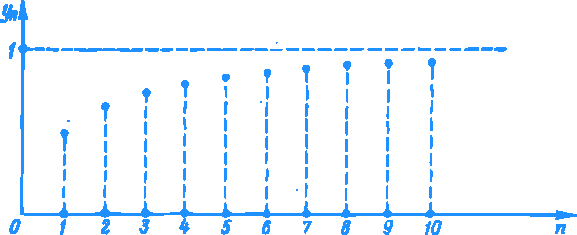
\includegraphics[width=0.9\textwidth]{figures/fig-03.pdf}
\caption{Image of the series \eqref{series-05}.}
\label{fig-03}
\end{figure}
 Later we shall talk about the \emph{geometric image} (or \emph{map}) of a numerical sequence. Let us take two coordinate axes, $x$ and $y$. We shall mark on the first axis integers $1, \, 2, \, 3, \ldots, n, \ldots$ and on the second axis, the corresponding terms of a sequence, i.e. the numbers $y_{1}, \, y_{2}, \, y_{3}, \ldots y_{n}, \ldots$. Then the sequence can be represented by a set of points $M (n, y_{n})$ on the coordinate plane. For example \fig{fig-02} images sequence \eqref{series-04}, \fig{fig-03} images sequence \eqref{series-05}, \fig{fig-04} images sequence \eqref{series-09}, and \fig{fig-05} images sequence \eqref{series-10}.
\begin{figure}[!h]
\centering
\begin{tikzpicture}[line cap=round,line join=round,>=triangle 45,x=1.0cm,y=3.5cm]
\foreach \x in {1,2,3,4,5,6,7,9}
\draw[shift={(\x,0)},color=black] (0pt,2pt) -- (0pt,-2pt) node[below] {\footnotesize $\x$};
\foreach \y in {-1,0,1}
\draw[shift={(0,\y)},color=black] (2pt,0pt) -- (-2pt,0pt) node[left] {\footnotesize $\y$};
\clip(-1.4,-1.1) rectangle (11.4,1.3);
\draw (-0.641960402073037,1.1784020472890375) node[anchor=north west] {$y_{n}$};
\draw (11,0) node[anchor=north west] {$n$};
\draw (10,-0.015) node[anchor=north west] {\footnotesize $10$};
\draw (8,-0.015) node[anchor=north west] {\footnotesize $8$};
\draw [->,line width=1.2pt,color=DarkGray] (0.,-1.0) -- (0.,1.2);
\draw [->,line width=1.2pt,color=DarkGray] (0.,0.) -- (11.2,0.);
\draw [line width=.75pt,dash pattern=on 3pt off 3pt,color=DarkGray] (0.,1.)-- (1.,1.);
\draw [line width=.75pt,dash pattern=on 3pt off 3pt,color=DarkGray] (1.,1.)-- (1.,0.);
\draw [line width=.75pt,dash pattern=on 3pt off 3pt,color=DarkGray] (0.,-1.)-- (2.,-1.);
\draw [line width=.75pt,dash pattern=on 3pt off 3pt,color=DarkGray] (2.,-1.)-- (2.,0.);
\draw [line width=.75pt,dash pattern=on 3pt off 3pt,color=DarkGray] (0.,0.3333333333333333)-- (3.,0.3333333333333333);
\draw [line width=.75pt,dash pattern=on 3pt off 3pt,color=DarkGray] (3.,0.3333333333333333)-- (3.,0.);
\draw [line width=.75pt,dash pattern=on 3pt off 3pt,color=DarkGray] (4.,0.)-- (4.,-0.3333333333333333);
\draw [line width=.75pt,dash pattern=on 3pt off 3pt,color=DarkGray] (4.,-0.3333333333333333)-- (0.,-0.3333333333333333);
\draw [line width=.75pt,dash pattern=on 3pt off 3pt,color=DarkGray] (0.,0.2)-- (5.,0.2);
\draw [line width=.75pt,dash pattern=on 3pt off 3pt,color=DarkGray] (5.,0.2)-- (5.,0.);
\draw [line width=.75pt,dash pattern=on 3pt off 3pt,color=DarkGray] (6.,0.)-- (6.,-0.2);
\draw [line width=.75pt,dash pattern=on 3pt off 3pt,color=DarkGray] (0.,-0.2)-- (6.,-0.2);
\draw [line width=.75pt,dash pattern=on 3pt off 3pt,color=DarkGray] (7.,0.14285714285714285)-- (7.,0.);
\draw [line width=.75pt,dash pattern=on 3pt off 3pt,color=DarkGray] (8.,-0.14285714285714285)-- (8.,0.);
\draw [line width=.75pt,dash pattern=on 3pt off 3pt,color=DarkGray] (9.,0.125)-- (9.,0.);
\draw [line width=.75pt,dash pattern=on 3pt off 3pt,color=DarkGray] (10.,-0.125)-- (10.,0.);
\begin{scriptsize}
\filldraw [IndianRed] (1.,1.) circle (2.5pt);
\filldraw [IndianRed] (2.,-1.) circle (2.5pt);
\filldraw [IndianRed] (3.,0.3333333333333333) circle (2.5pt);
\filldraw [IndianRed] (4.,-0.3333333333333333) circle (2.5pt);
\filldraw [IndianRed] (5.,0.2) circle (2.5pt);
\filldraw [IndianRed] (6.,-0.2) circle (2.5pt);
\filldraw [IndianRed] (7.,0.14285714285714285) circle (2.5pt);
\filldraw [IndianRed] (8.,-0.14285714285714285) circle (2.5pt);
\filldraw [DodgerBlue] (1.,0.) circle (2.5pt);
\filldraw [DodgerBlue] (2.,0.) circle (2.5pt);
\filldraw [DodgerBlue] (3.,0.) circle (2.5pt);
\filldraw [DodgerBlue] (4.,0.) circle (2.5pt);
\filldraw [DodgerBlue] (5.,0.) circle (2.5pt);
\filldraw [DodgerBlue] (6.,0.) circle (2.5pt);
\filldraw [DodgerBlue] (7.,0.) circle (2.5pt);
\filldraw [DodgerBlue] (8.,0.) circle (2.5pt);
\filldraw [DodgerBlue] (9.,0.) circle (2.5pt);
\filldraw [DodgerBlue] (10.,0.) circle (2.5pt);
\filldraw [DodgerBlue] (0.,0.3333333333333333) circle (2.5pt);
\filldraw [DodgerBlue] (0.,-0.3333333333333333) circle (2.5pt);
\filldraw [DodgerBlue] (0.,0.2) circle (2.5pt);
\filldraw [DodgerBlue] (0.,-0.2) circle (2.5pt);
\filldraw [DodgerBlue] (0.,1.) circle (2.5pt);
\filldraw [DodgerBlue] (0.,0.) circle (2.5pt);
\filldraw [DodgerBlue] (0.,-1.) circle (2.5pt);
\filldraw [IndianRed] (9.,0.125) circle (2.5pt);
\filldraw [IndianRed] (10.,-0.125) circle (2.5pt);
\end{scriptsize}
\end{tikzpicture}
%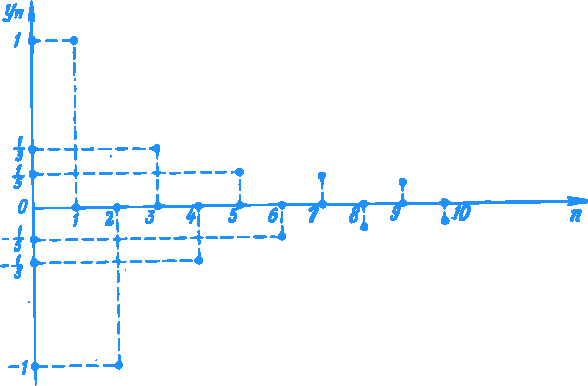
\includegraphics[width=0.9\textwidth,angle=-1]{figures/fig-04.pdf}
\caption{Series in equation \eqref{series-09} visualised.}
\label{fig-04}

\end{figure}
\begin{figure}[!h]
\centering
\begin{tikzpicture}[line cap=round,line join=round,>=triangle 45,x=1.0cm,y=3.5cm]
\foreach \x in {1,2,3,4,5,6,7,8,9,10}
\draw[shift={(\x,0)},color=black] (0pt,2pt) -- (0pt,-2pt) node[below] {\footnotesize $\x$};
\foreach \y in {0,1}
\draw[shift={(0,\y)},color=black] (2pt,0pt) -- (-2pt,0pt) node[left] {\footnotesize $\y$};
\draw[shift={(0,0.33)},color=black]  (2pt,0pt) -- (-2pt,0pt) node[left] {\footnotesize $\dfrac{1}{3}$};
\draw[shift={(0,0.66)},color=black]  (2pt,0pt) -- (-2pt,0pt) node[left] {\footnotesize $\dfrac{2}{3}$};
\clip(-0.9,-0.12) rectangle (11,1.3);
\draw (-0.6,1.2) node[anchor=north west] {$y_{n}$};
\draw (10.457277999784147,-0.03) node[anchor=north west] {$n$};
\draw [->,line width=1.2pt,color=DarkGray] (0.,0.) -- (0.,1.25);
\draw [->,line width=1.2pt,color=DarkGray] (0.,0.) -- (11.,0.);
\draw [line width=.75pt,dash pattern=on 3pt off 3pt,color=DarkGray] (0.,1.)-- (1.,1.);
\draw [line width=.75pt,dash pattern=on 3pt off 3pt,color=DarkGray] (1.,1.)-- (1.,0.);
\draw [line width=1pt,dash pattern=on 3pt off 3pt,color=IndianRed,domain=0:11] plot(\x,{(--1.-0.*\x)/1.});
\draw [line width=.75pt,dash pattern=on 3pt off 3pt,color=DarkGray] (2.,0.6666666666666666)-- (2.,0.);
\draw [line width=.75pt,dash pattern=on 3pt off 3pt,color=DarkGray] (2.,0.6666666666666666)-- (0.,0.6666666666666666);
\draw [line width=.75pt,dash pattern=on 3pt off 3pt,color=DarkGray] (3.,0.3333333333333333)-- (0.,0.3333333333333333);
\draw [line width=.75pt,dash pattern=on 3pt off 3pt,color=DarkGray] (3.,0.3333333333333333)-- (3.,0.);
\draw [line width=.75pt,dash pattern=on 3pt off 3pt,color=DarkGray] (4.,0.75)-- (4.,0.);
\draw [line width=.75pt,dash pattern=on 3pt off 3pt,color=DarkGray] (5.,0.2)-- (5.,0.);
\draw [line width=.75pt,dash pattern=on 3pt off 3pt,color=DarkGray] (6.,0.8571428571428571)-- (6.,0.);
\draw [line width=.75pt,dash pattern=on 3pt off 3pt,color=DarkGray] (7.,0.14285714285714285)-- (7.,0.);
\draw [line width=.75pt,dash pattern=on 3pt off 3pt,color=DarkGray] (8.,0.8888888888888888)-- (8.,0.);
\draw [line width=.75pt,dash pattern=on 3pt off 3pt,color=DarkGray] (9.,0.1111111111111111)-- (9.,0.);
\draw [line width=.75pt,dash pattern=on 3pt off 3pt,color=DarkGray] (10.,0.9)-- (10.,0.);
\begin{scriptsize}
\filldraw [IndianRed] (1.,1.) circle (2.5pt);
\filldraw [DodgerBlue] (1.,0.) circle (2.5pt);
\filldraw [DodgerBlue] (2.,0.) circle (2.5pt);
\filldraw [DodgerBlue] (3.,0.) circle (2.5pt);
\filldraw [DodgerBlue] (4.,0.) circle (2.5pt);
\filldraw [DodgerBlue] (5.,0.) circle (2.5pt);
\filldraw [DodgerBlue] (6.,0.) circle (2.5pt);
\filldraw [DodgerBlue] (7.,0.) circle (2.5pt);
\filldraw [DodgerBlue] (8.,0.) circle (2.5pt);
\filldraw [DodgerBlue] (9.,0.) circle (2.5pt);
\filldraw [DodgerBlue] (10.,0.) circle (2.5pt);
\filldraw [DodgerBlue] (0.,1.) circle (2.5pt);
\filldraw [IndianRed] (2.,0.6666666666666666) circle (2.5pt);
\filldraw [IndianRed] (3.,0.3333333333333333) circle (2.5pt);
\filldraw [IndianRed] (4.,0.75) circle (2.5pt);
\filldraw [DodgerBlue] (0.,0.6666666666666666) circle (2.5pt);
\filldraw [DodgerBlue] (0.,0.3333333333333333) circle (2.5pt);
\filldraw [IndianRed] (5.,0.2) circle (2.5pt);
\filldraw [IndianRed] (6.,0.8571428571428571) circle (2.5pt);
\filldraw [IndianRed] (7.,0.14285714285714285) circle (2.5pt);
\filldraw [IndianRed] (8.,0.8888888888888888) circle (2.5pt);
\filldraw [IndianRed] (9.,0.1111111111111111) circle (2.5pt);
\filldraw [IndianRed] (10.,0.9) circle (2.5pt);
\end{scriptsize}
\end{tikzpicture}
%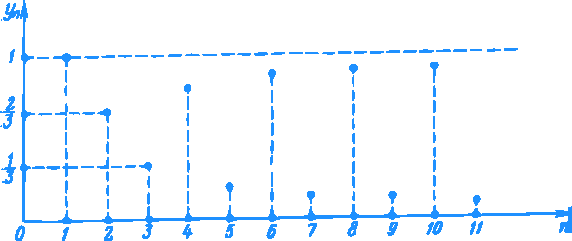
\includegraphics[width=0.9\textwidth,angle=-1]{figures/fig-05.pdf}
\caption{Series in equation \eqref{series-10} visualised.}
\label{fig-05}
\end{figure}

As a matter of fact, there are other types of geometry images of a numerical sequence. Let us retain, for example only one coordinate $y$-axis and plot on it points  $y_{1}, \, y_{2}, \, y_{3}, \ldots y_{n}, \ldots$ which map the terms of a sequence. In \fig{fig-06} this method of mapping is illustrated for the sequences that have been shown in \fig{fig-02}-\fig{fig-05}. One has to admit that the latter method is less descriptive in comparison with the former method.
\begin{figure}[!h]
\centering
\begin{tikzpicture}[baseline=1cm,line cap=round,line join=round,>=triangle 45,x=2.5cm,y=2.0cm]
\foreach \x in {0,1,2,3,4}
\draw[shift={(\x,0)},color=black] (0pt,2pt) -- (0pt,-2pt) node[below] {\footnotesize $\x$};
\clip(-0.3,-0.3) rectangle (5.,0.52);
\draw (4.212511655558804,0.008475512540077454) node[anchor=north west] {$y$};
\draw [->,line width=1.2pt,color=DarkGray] (0.,0.) -- (4.6,0.);
\draw (1.9,0.35) node[anchor=north west] {$y_{4}$};
\draw (2.88,0.35) node[anchor=north west] {$y_{9}$};
\draw (1.6,0.35) node[anchor=north west] {$y_{3}$};
\draw (1.3171801125876044,0.35) node[anchor=north west] {$y_{2}$};
\draw (0.9,0.35) node[anchor=north west] {$y_{1}$};
\draw (-0.1,0.5) node[anchor=north west,color=IndianRed] {\textit{Sequence} (4)};
\begin{scriptsize}
\filldraw [DodgerBlue] (11.,0.) circle (2.5pt);
\filldraw [DodgerBlue] (1.,0.) circle (2.5pt);
\filldraw [DodgerBlue] (2.,0.) circle (2.5pt);
\filldraw [DodgerBlue] (3.,0.) circle (2.5pt);
\filldraw [DodgerBlue] (4.,0.) circle (2.5pt);
\filldraw [DodgerBlue] (0.,0.) circle (2.5pt);
\filldraw [DodgerBlue] (1.,0.) circle (2.5pt);
\filldraw [DodgerBlue] (1.41,0.) circle (2.5pt);
\filldraw [DodgerBlue] (1.73,0.) circle (2.5pt);
\filldraw [DodgerBlue] (2.,0.) circle (2.5pt);
\filldraw [DodgerBlue] (2.24,0.) circle (2.5pt);
\filldraw [DodgerBlue] (2.45,0.) circle (2.5pt);
\filldraw [DodgerBlue] (2.65,0.) circle (2.5pt);
\filldraw [DodgerBlue] (2.83,0.) circle (2.5pt);
\filldraw [DodgerBlue] (3.,0.) circle (2.5pt);
\filldraw [DodgerBlue] (3.16,0.) circle (2.5pt);
\filldraw [DodgerBlue] (3.32,0.) circle (2.5pt);
\filldraw [DodgerBlue] (3.46,0.) circle (2.5pt);
\filldraw [DodgerBlue] (3.61,0.) circle (2.5pt);
\filldraw [DodgerBlue] (3.74,0.) circle (2.5pt);
\filldraw [DodgerBlue] (3.87,0.) circle (2.5pt);
\filldraw [DodgerBlue] (4.,0.) circle (2.5pt);
\filldraw [DodgerBlue] (4.12,0.) circle (2.5pt);
\filldraw [DodgerBlue] (1.,0.) circle (2.5pt);
\filldraw [DodgerBlue] (1.41,0.) circle (2.5pt);
\filldraw [DodgerBlue] (1.73,0.) circle (2.5pt);
\filldraw [DodgerBlue] (2.,0.) circle (2.5pt);
\filldraw [DodgerBlue] (2.24,0.) circle (2.5pt);
\filldraw [DodgerBlue] (2.45,0.) circle (2.5pt);
\filldraw [DodgerBlue] (2.65,0.) circle (2.5pt);
\filldraw [DodgerBlue] (2.83,0.) circle (2.5pt);
\filldraw [DodgerBlue] (3.,0.) circle (2.5pt);
\filldraw [DodgerBlue] (3.16,0.) circle (2.5pt);
\filldraw [DodgerBlue] (3.32,0.) circle (2.5pt);
\filldraw [DodgerBlue] (3.46,0.) circle (2.5pt);
\filldraw [DodgerBlue] (3.61,0.) circle (2.5pt);
\filldraw [DodgerBlue] (3.74,0.) circle (2.5pt);
\filldraw [DodgerBlue] (3.87,0.) circle (2.5pt);
\filldraw [DodgerBlue] (4.,0.) circle (2.5pt);
\filldraw [DodgerBlue] (4.12,0.) circle (2.5pt);
\end{scriptsize}
\end{tikzpicture}

%\\[5pt] %\hspace{5pt}
\begin{tikzpicture}[line cap=round,line join=round,>=triangle 45,x=10.5cm,y=2.0cm]
\foreach \x in {0,0.5,0.6,0.8,0.9,1}
\draw[shift={(\x,0)},color=black] (0pt,2pt) -- (0pt,-2pt) node[below] {\footnotesize $\x$};
\clip(-0.02,-0.2) rectangle (1.3,0.4);
\draw (4.214177852337174,0.002715213130875362) node[anchor=north west] {$y$};
\draw (0.80,0.1) node[above] {$y_{4}$};
\draw (2.9578364575840723,0.1) node[above] {$y_{9}$};
\draw (0.75,0.1) node[above] {$y_{3}$};
\draw (0.67,0.1) node[above] {$y_{2}$};
\draw (0.5,0.1) node[above] {$y_{1}$};
\draw (0.0702198757690745,0.4) node[anchor=north west,color=IndianRed] {\textit{Sequence}\,\, (5)};
\draw [->,line width=1.2pt,color=DarkGray] (0.,0.) -- (1.1,0.);
\begin{scriptsize}
\filldraw [DodgerBlue] (0.5,0.) circle (2.5pt);
\filldraw [DodgerBlue] (0.667,0.) circle (2.5pt);
\filldraw [DodgerBlue] (0.75,0.) circle (2.5pt);
\filldraw [DodgerBlue] (0.8,0.) circle (2.5pt);
\filldraw [DodgerBlue] (0.833,0.) circle (2.5pt);
\filldraw [DodgerBlue] (0.857,0.) circle (2.5pt);
\filldraw [DodgerBlue] (0.875,0.) circle (2.5pt);
\filldraw [DodgerBlue] (0.889,0.) circle (2.5pt);
\filldraw [DodgerBlue] (0.9,0.) circle (2.5pt);
\filldraw [DodgerBlue] (0.917,0.) circle (2.5pt);
\filldraw [DodgerBlue] (0.923,0.) circle (2.5pt);
\filldraw [DodgerBlue] (0.933,0.) circle (2.5pt);
\filldraw [DodgerBlue] (0.941,0.) circle (2.5pt);
\filldraw [DodgerBlue] (0.,0.) circle (2.5pt);
\filldraw [DodgerBlue] (0.,0.) circle (2.5pt);
\end{scriptsize}
\end{tikzpicture}
%\\[5pt]%\hspace{5pt} 
\begin{tikzpicture}[line cap=round,line join=round,>=triangle 45,x=6cm,y=2.0cm]
\foreach \x in {-1,-0.8,-0.6,-0.4,-0.2,0,0.2,0.4,0.6,0.8,1}
\draw[shift={(\x,0)},color=black] (0pt,2pt) -- (0pt,-2pt) node[below] {\footnotesize $\x$};
\clip(-1.1,-0.3) rectangle (1.1,0.7);
\draw (4.213643364971578,0.3) node[anchor=north west] {$y$};
\draw (-0.38,0.3) node[anchor=north west] {$y_{4}$};
\draw (2.9579444591417623,0.3) node[anchor=north west] {$y_{9}$};
\draw (0.28,0.3) node[anchor=north west] {$y_{3}$};
\draw (-1.0293879928920922,0.3) node[anchor=north west] {$y_{2}$};
\draw (0.9580619019078557,0.3) node[anchor=north west] {$y_{1}$};
\draw (-0.9636724914554541,0.55) node[anchor=north west,color=IndianRed] {\textit{Sequence} (9)};
\draw [->,line width=1.2pt,color=DarkGray] (0.,0.) -- (-1.1,0.);
\draw [->,line width=1.2pt,color=DarkGray] (0.,0.) -- (1.1,0.);
\draw (0.16,.3) node[anchor=north west] {$y_{5}$};
\draw (-0.23192150248532134,.3) node[anchor=north west] {$y_{6}$};
\begin{scriptsize}
\filldraw [DodgerBlue](1.,0.) circle (2.5pt);
\filldraw [DodgerBlue](-1.,0.) circle (2.5pt);
\filldraw [DodgerBlue](0.333,0.) circle (2.5pt);
\filldraw [DodgerBlue](-0.333,0.) circle (2.5pt);
\filldraw [DodgerBlue](0.2,0.) circle (2.5pt);
\filldraw [DodgerBlue](-0.2,0.) circle (2.5pt);
\filldraw [DodgerBlue](0.143,0.) circle (2.5pt);
\filldraw [DodgerBlue](-0.143,0.) circle (2.5pt);
\filldraw [DodgerBlue](0.111,0.) circle (2.5pt);
\filldraw [DodgerBlue](-0.111,0.) circle (2.5pt);
\filldraw [DodgerBlue](0.091,0.) circle (2.5pt);
\filldraw [DodgerBlue](-0.091,0.) circle (2.5pt);
\filldraw [DodgerBlue](1.,0.) circle (2.5pt);
\filldraw [DodgerBlue](-1.,0.) circle (2.5pt);
\filldraw [DodgerBlue](0.333,0.) circle (2.5pt);
\filldraw [DodgerBlue](-0.333,0.) circle (2.5pt);
\filldraw [DodgerBlue](0.2,0.) circle (2.5pt);
\filldraw [DodgerBlue](-0.2,0.) circle (2.5pt);
\filldraw [DodgerBlue](0.143,0.) circle (2.5pt);
\filldraw [DodgerBlue](-0.143,0.) circle (2.5pt);
\filldraw [DodgerBlue](0.111,0.) circle (2.5pt);
\filldraw [DodgerBlue](-0.111,0.) circle (2.5pt);
\filldraw [DodgerBlue](0.091,0.) circle (2.5pt);
\filldraw [DodgerBlue](-0.091,0.) circle (2.5pt);
\end{scriptsize}
\end{tikzpicture}%\\[5pt]
\begin{tikzpicture}[line cap=round,line join=round,>=triangle 45,x=7cm,y=1.5cm]
\foreach \x in {0,1}
\draw[shift={(\x,0)},color=black] (0pt,2pt) -- (0pt,-2pt) node[below] {\footnotesize $\x$};
\clip(-0.9,-0.45) rectangle (1.2,1.3);
\draw (10.457277999784147,-0.03) node[anchor=north west] {$n$};
\draw [->,line width=1.2pt,color=DarkGray] (0.,0.) -- (1.1,0.);
\draw (1,0.15) node[above] {$y_{1}$};
\draw (0.67,0.15) node[above] {$y_{2}$};
\draw (0.66,0) node[below] {\footnotesize $\frac{2}{3}$};
\draw (0.33,0) node[below] {\footnotesize $\frac{1}{3}$};
\draw (0.34,0.15) node[above] {$y_{3}$};
\draw (.75,0.15) node[above] {$y_{4}$};
\draw (0.22,0.15) node[above] {$y_{5}$};
\draw (0.88,0.15) node[above] {$y_{6}$};
\draw (0.14,0.15) node[above] {$y_{7}$};
\draw (0,0.85) node[anchor=north west,color=IndianRed] {\textit{Sequence} (10)};
\begin{scriptsize}
\filldraw [DodgerBlue] (1,0) circle (2.5pt);
\filldraw [DodgerBlue] (0.6666666666666666,0) circle (2.5pt);
\filldraw [DodgerBlue] (0.3333333333333333,0) circle (2.5pt);
\filldraw [DodgerBlue] (0.75,0) circle (2.5pt);
\filldraw [DodgerBlue] (0.2,0) circle (2.5pt);
\filldraw [DodgerBlue] (0.85,0) circle (2.5pt);
\filldraw [DodgerBlue] (0.14,0) circle (2.5pt);
\filldraw [DodgerBlue] (0.88,0) circle (2.5pt);
\filldraw [DodgerBlue] (0.11,0) circle (2.5pt);
\filldraw [DodgerBlue] (0.9,0) circle (2.5pt);
\end{scriptsize}
\end{tikzpicture}
%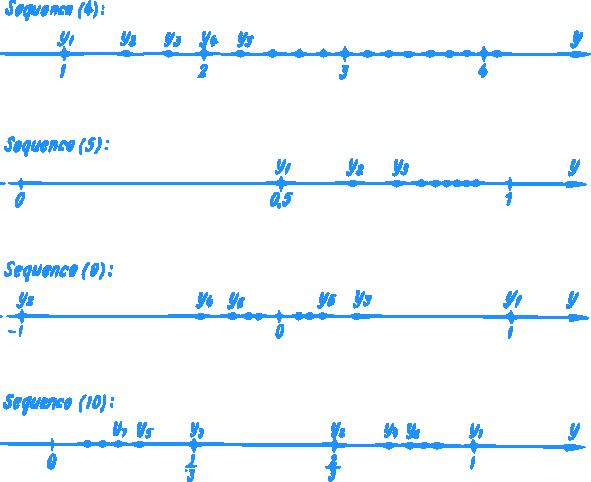
\includegraphics[width=0.9\textwidth]{figures/fig-06.pdf}
\caption{Mapping the sequences along a line.}
\label{fig-06}
\end{figure}

\rdr But in the case of sequences \eqref{series-04} and \eqref{series-05} the seond method looks rather obvious.

\athr It can be explained by specific features of those sequences. Look at them closer.

\rdr The terms of sequences  \eqref{series-04} and \eqref{series-05} possess the following property: each term is greater than the preceding term
\begin{equation*}%
y_{1} < y_{2} < y_{3}, \ldots < y_{n} < \ldots
\end{equation*}
It means that all the terms are arranged on the $y$-axis according to their serial numbers. As far as I know, such sequence, are called \emph{increasing}.

\athr A more general case is that of \emph{non-decreasing} sequences provided we add the equality sign to the above series of inequalities.
\begin{mytheo}{Definition}
A sequence ($y_{n}$) is called nondecreasing if
\begin{equation*}%
y_{1} \leqslant y_{2} \leqslant y_{3}, \ldots \leqslant y_{n} \leqslant \ldots
\end{equation*}
A sequence ($y_{n}$) is called non-increasing if
\begin{equation*}%
y_{1} \geqslant y_{2} \geqslant y_{3}, \ldots \geqslant y_{n} \geqslant \ldots
\end{equation*}
Non-decreasing and non-increasing sequences come under the name of monotonic sequences.
\end{mytheo}
Please, identify monotonic sequences among examples \eqref{series-01} -\eqref{series-13}.

\rdr Sequences \eqref{series-01}, \eqref{series-02}, \eqref{series-03}, \eqref{series-04}, \eqref{series-05}, \eqref{fibonacci}, \eqref{series-12}, and \eqref{series-13} are nondecreasing, while \eqref{series-06} and \eqref{series-07} are non-increasing. Sequences \eqref{series-08}, \eqref{series-09}, and \eqref{series-10} are not monotonic.

\athr Let us formulate one more definition.
\begin{mytheo}{Definition}
A sequence ($y_{n}$) is bounded if there are two numbers $A$ and $B$
labelling the range which encloses all the terms of a sequence
\begin{equation*}%
A \leqslant y_{n} \leqslant B \,\, (n = 1, \, 2, \, 3, \, \ldots)
\end{equation*}
\end{mytheo}

If it is impossible to identify such two numbers (or, in particular, one can find only one of the two such numbers, either the least or the greatest), such a sequence is \emph{unbounded}. Do you find bounded sequences among our examples? 

\rdr Apparently, \eqref{series-05} is bounded. 

\athr Find the numbers $A$ and $B$ for it.

\rdr $A=1/2, \, B= 1$.

\athr Of course, but if there exists even one pair of $A$ and $B$, one may find any number of such pairs. You could say, for example, that $A= 0, \, B= 2$, or $A=-100, \, B = 100$, etc., and be equally right.

\rdr Yes, but my numbers are more accurate.

\athr From the viewpoint of the bounded sequence definition, my numbers $A$ and $B$ are not Letter and not worse than yours. However, your last sentence is peculiar. What do you mean by saying ``more accurate?''

\rdr My $A$ is apparently the greatest of all possible lower bounds, while my $B$ is the least of all possible upper hounds.

\athr The first part of your statement is doubtlessly correct, while the second part of it, concerning $B$, is not so self-explanatory. It needs proof.

\rdr But it seemed	rather obvious. Because all the terms of \eqref{series-05} increase gradually, and evidently tend to unity, always remaining less than unity.

\athr Well, it is right. But it is not yet evident that $B = 1$ is the least number for which $y_{n} \leqslant B$ is valid for all $n$: I stress the point again: your statement is not self-evident, it needs proof.

I shall note also that ``self-evidence'' of your statement about $B = 1$ is nothing but your subjective impression; it is not a mathematically substantiated corollary.


\rdr But how to prove that $B = 1$ is, in this particular case, the least of all possible upper bounds?

\athr Yes, it can be proved. But let us not move too fast and by all means beware of excessive reliance on so-called self-evident impressions. The warning becomes even more important in the light of the fact that the bounded- ness of a sequence does not imply at all that the greatest $A$ or the least $B$ must be known explicitly.

Now, let us get back to our sequences and find other examples of bounded sequences.	 .

\rdr Sequence \eqref{series-07} is also bounded (one can easily find $A = 0, \, B = 1$). Finally, bounded sequences are \eqref{series-09} (e.g. $A=-1, \,B= 1$), \eqref{series-10} (e.g. $A=0, \, B= 1$), and \eqref{series-13} (e.g. $A = 3, \, B = 4$). The remaining' sequences are un-bounded.

\athr You are quite right. Sequences \eqref{series-05}, \eqref{series-07}, \eqref{series-09}, \eqref{series-10}, and \eqref{series-13} are bounded. Note that \eqref{series-05}, \eqref{series-07}, and \eqref{series-13} are bounded and at the same time monotonic. Don't you feel that this fact is somewhat puzzling?

\rdr What's puzzling about it?

\athr Consider, for example, sequence \eqref{series-05}. Note that each subsequent term is greater than the preceding one. I repeat, each term! But the sequence contains an infinite number of terms. Hence, if we follow the sequence far enough, we shall see as many terms with increased magnitude (compared to the preceding term) as we wish. Nevertheless, these values will never go beyond a certain ``boundary'', which in this case is unity. Doesn't it puzzle you?

\rdr Well, generally speaking, it does. But I notice that we add to each preceding term an increment which gradually becomes less and less.

\athr Yes, it is true. But this condition is obviously insufficient to make such a sequence bounded. Take, for example, sequence \eqref{series-04}. Here again the ``increments'' added to each term of the sequence gradually decrease; nevertheless, the sequence is not bounded.

\rdr We must conclude, therefore, that in \eqref{series-05} these ``increments'' diminish faster than in \eqref{series-04}.

\athr All the same, you have to agree that it is not immediately clear that these ``increments'' may decrease at a rate resulting in the boundedness of a sequence.

\rdr Of course, I agree with that.

\athr The possibility of infinite but bounded sets was not known, for example, to ancient Greeks. Suffice it to recall the famous paradox about Achilles chasing a turtle.

Let us assume that Achilles and the turtle are initially separated by a distance of \SI{1}{\kilo\meter}, Achilles moves to times faster than the turtle. Ancient Greeks reasoned like this: during the time Achilles covers \SI{1}{\kilo\meter} the turtle covers \SI{100}{\meter}. By the time Achilles has covered these \SI{100}{\meter}, the turtle will have made another \SI{10}{\meter}, and before Achilles has covered these \SI{10}{\meter}, the turtle will have made \SI{1}{\meter} more, and so on. Out of these considerations a paradoxical conclusion was derived that Achilles could never catch up with the turtle.

This ``paradox'' shows that ancient Greeks failed to grasp the fact that a monotonic sequence may be bounded.

\rdr One has to agree that the presence of both the monotonicity and boundedness is something not so simple to understand.

\athr Indeed, this is not so simple. It brings us close to a discussion on the limit of sequence. The point is that if a sequence is both monotonic and bounded, it should necessarily have a limit.

Actually, this point can be considered as the ``beginning'' of calculus.
}